\documentclass[aps,pra,twocolumn,10pt]{revtex4-1}
\usepackage{amssymb}
\usepackage{amsfonts}
\usepackage[fleqn,tbtags]{amsmath}
\usepackage{graphicx} 


\begin{document}

\title{Quantum Annealing for Air Traffic Management}
\author{Tobias Stollenwerk}
\affiliation{German Aerospace Center, Linder H\"ohe, 51147 Cologne, Germany}
\author{Bryan O'Gorman},
\author{Salvatore Mandr\`{a}}
\author{Eleanor G. Rieffel}
%\author{Davide Venturelli},
%\author{Olga Rodionova},
%\author{Hok K. Ng},
%\author{Banavar Sridhar},
\affiliation{NASA Ames, Moffet Blvd, Mountain View, CA 94035, USA}
\date{\today}

\maketitle


%%%%%%%%%%%%%%%%%%%%%%%%%%%%%%%%%%%%%%%%%%%%%%%%%%%%%%%%%%%%%%%%%%%%%%%%%%%%%%
%%%%%%%%%%%%%%%%%%%%%%%%%%%%%%%%%%%%%%%%%%%%%%%%%%%%%%%%%%%%%%%%%%%%%%%%%%%%%%
%%%%%%%%%%%%%%%%%%%%%%%%%%%%%%%%%%%%%%%%%%%%%%%%%%%%%%%%%%%%%%%%%%%%%%%%%%%%%%
%%%%%%%%%%%%%%%%%%%%%%%%%%%%%%%%%%%%%%%%%%%%%%%%%%%%%%%%%%%%%%%%%%%%%%%%%%%%%%
%%%%%%%%%%%%%%%%%%%%%%%%%%%%%%%%%%%%%%%%%%%%%%%%%%%%%%%%%%%%%%%%%%%%%%%%%%%%%%
\section{Introduction}


%%%%%%%%%%%%%%%%%%%%%%%%%%%%%%%%%%%%%%%%%%%%%%%%%%%%%%%%%%%%%%%%%%%%%%%%%%%%%%
%%%%%%%%%%%%%%%%%%%%%%%%%%%%%%%%%%%%%%%%%%%%%%%%%%%%%%%%%%%%%%%%%%%%%%%%%%%%%%
%%%%%%%%%%%%%%%%%%%%%%%%%%%%%%%%%%%%%%%%%%%%%%%%%%%%%%%%%%%%%%%%%%%%%%%%%%%%%%
%%%%%%%%%%%%%%%%%%%%%%%%%%%%%%%%%%%%%%%%%%%%%%%%%%%%%%%%%%%%%%%%%%%%%%%%%%%%%%
%%%%%%%%%%%%%%%%%%%%%%%%%%%%%%%%%%%%%%%%%%%%%%%%%%%%%%%%%%%%%%%%%%%%%%%%%%%%%%
\section{Problem Description}
The problem at hand is the deconflicting of transatlantic wind-optimal trajectories.
As it was done in \cite{rodionova16} we are using the same wind-optimal trajectories of a single day, July 29 2012.
These wind-optimal trajectories are given as
${\left(\mathbf{x}_i\right)}_{i=1}^n$, 
where 
$\mathbf{x}_i = {\left(x_{i,t}\right)}_{t=t_{i,0}}^{t_{i,1}}$ 
and 
$x_{i, t}$ is the location (as latitude, longitude, and altitude) of the $i$th flight at time $t$.
The times $t_{i,0}$ and $t_{i, 1}$ are the times at which the wind-optimal trajectory for the $i$th flight begins and ends, respectively.
Furthermore, the times are given in units of one minutes $T_i = \left(t_{i, 0}, t_{i, 0} + 1, \ldots, t_{i, 1}\right)$.
Each flight $i$ is at a constant speed $v_i$, to within (classical) machine precision.

A conflict between two flights is defined as a pair of trajectory points which are too close to each other in space and time.
\begin{equation} \label{eqn:conflicting_trajectory_points}
    \{ (x_{i, t},  x_{j, t'}) \; | \; \mathcal{D} (x_{i, t}, x_{j, t'}) < \Delta_x ,  |t - t'| < \Delta_t \} \; ,
\end{equation}
where $\mathcal{D}(x, y)$ is the spatial distance between two points $x$ and $y$ given as latitude, longitude and altitude.
Following \cite{rodionova16}, the space threshold is $\Delta_x = 3$ nautical miles and the time threshold is $\Delta_t = 3$ minutes.
In this paper, we consider the following means to deconflict the trajectories:
First, we can delay each flight $i$ at departure time by a departure delay $d_i$
\begin{equation*}
    x_{i, t} \to x_{i, t + d_i} \quad \forall \; t \in T_{i}
\end{equation*}

Second, we can avoid a conflict by maneuvers of both involved flights.
We assume, however, that the maneuvers will not introduce new conflicts. 
In doing so, these maneuvers can be view as resulting in time shifts only.

%%%%%%%%%%%%%%%%%%%%%%%%%%%%%%%%%%%%%%%%%%%%%%%%%%%%%%%%%%%%%%%%%%%%%%%%%%%%%%
%%%%%%%%%%%%%%%%%%%%%%%%%%%%%%%%%%%%%%%%%%%%%%%%%%%%%%%%%%%%%%%%%%%%%%%%%%%%%%
%%%%%%%%%%%%%%%%%%%%%%%%%%%%%%%%%%%%%%%%%%%%%%%%%%%%%%%%%%%%%%%%%%%%%%%%%%%%%%
\subsection{Classical Preprocessing}
It is beneficial to reduce the data to conflicting regions in space and decoupling the spacial and temporal components of the problem.
As a first step, we detect all pairs of trajectory points which are separated by a spacial distance below $\Delta_x$ 
\begin{equation*}
    \{ (x_{i, t},  x_{j, t'}) \; | \; \mathcal{D} (x_{i, t}, x_{j, t'}) < \Delta_x \} \; ,
\end{equation*}
Two spatially conflicting trajectory points might never become conflicting in time if the corresponding times are far apart.
By introducing a constant maximum delay $D_{max}$ we can dismiss all spatial conflicts which can never become conflicting in time
\begin{equation*}
    \{ (x_{i, t},  x_{j, t'}) \; | \; \mathcal{D} (x_{i, t}, x_{j, t'}) < \Delta_x , |t-t'| \geq \Delta_t + D_\text{max} \} \; .
\end{equation*}
With this, we are left with a set of potentially conflicting pairs of trajectory points
\begin{equation*}
    C^{ij}_0 = \{ (x_{i, t},  x_{j, t'}) \; | \; \mathcal{D} (x_{i, t}, x_{j, t'}) < \Delta_x , |t-t'| < \Delta_t + D_\text{max} \} \; .
\end{equation*}

As a next step, we group together conflicting trajectory point pairs which are subsequent in time
\begin{align*}
    C^{ij}_\parallel = \{ ((x_{i, t},  x_{j, t'}),  (x_{i, s},  x_{j, s'})) \; | \; & (x_{i, t},  x_{j, t'}) \in C^{ij}_0, \\
                                                                                    & (x_{i, s},  x_{j, s'}) \in C^{ij}_0, \\ 
                                                                                    & |t - s| < \Delta'_t,  \\
                                                                                    & |t' - s'| < \Delta'_t \}
\end{align*}
where we set $\Delta'_t = 2$ minutes.

\begin{figure}[t]
    \begin{center}
        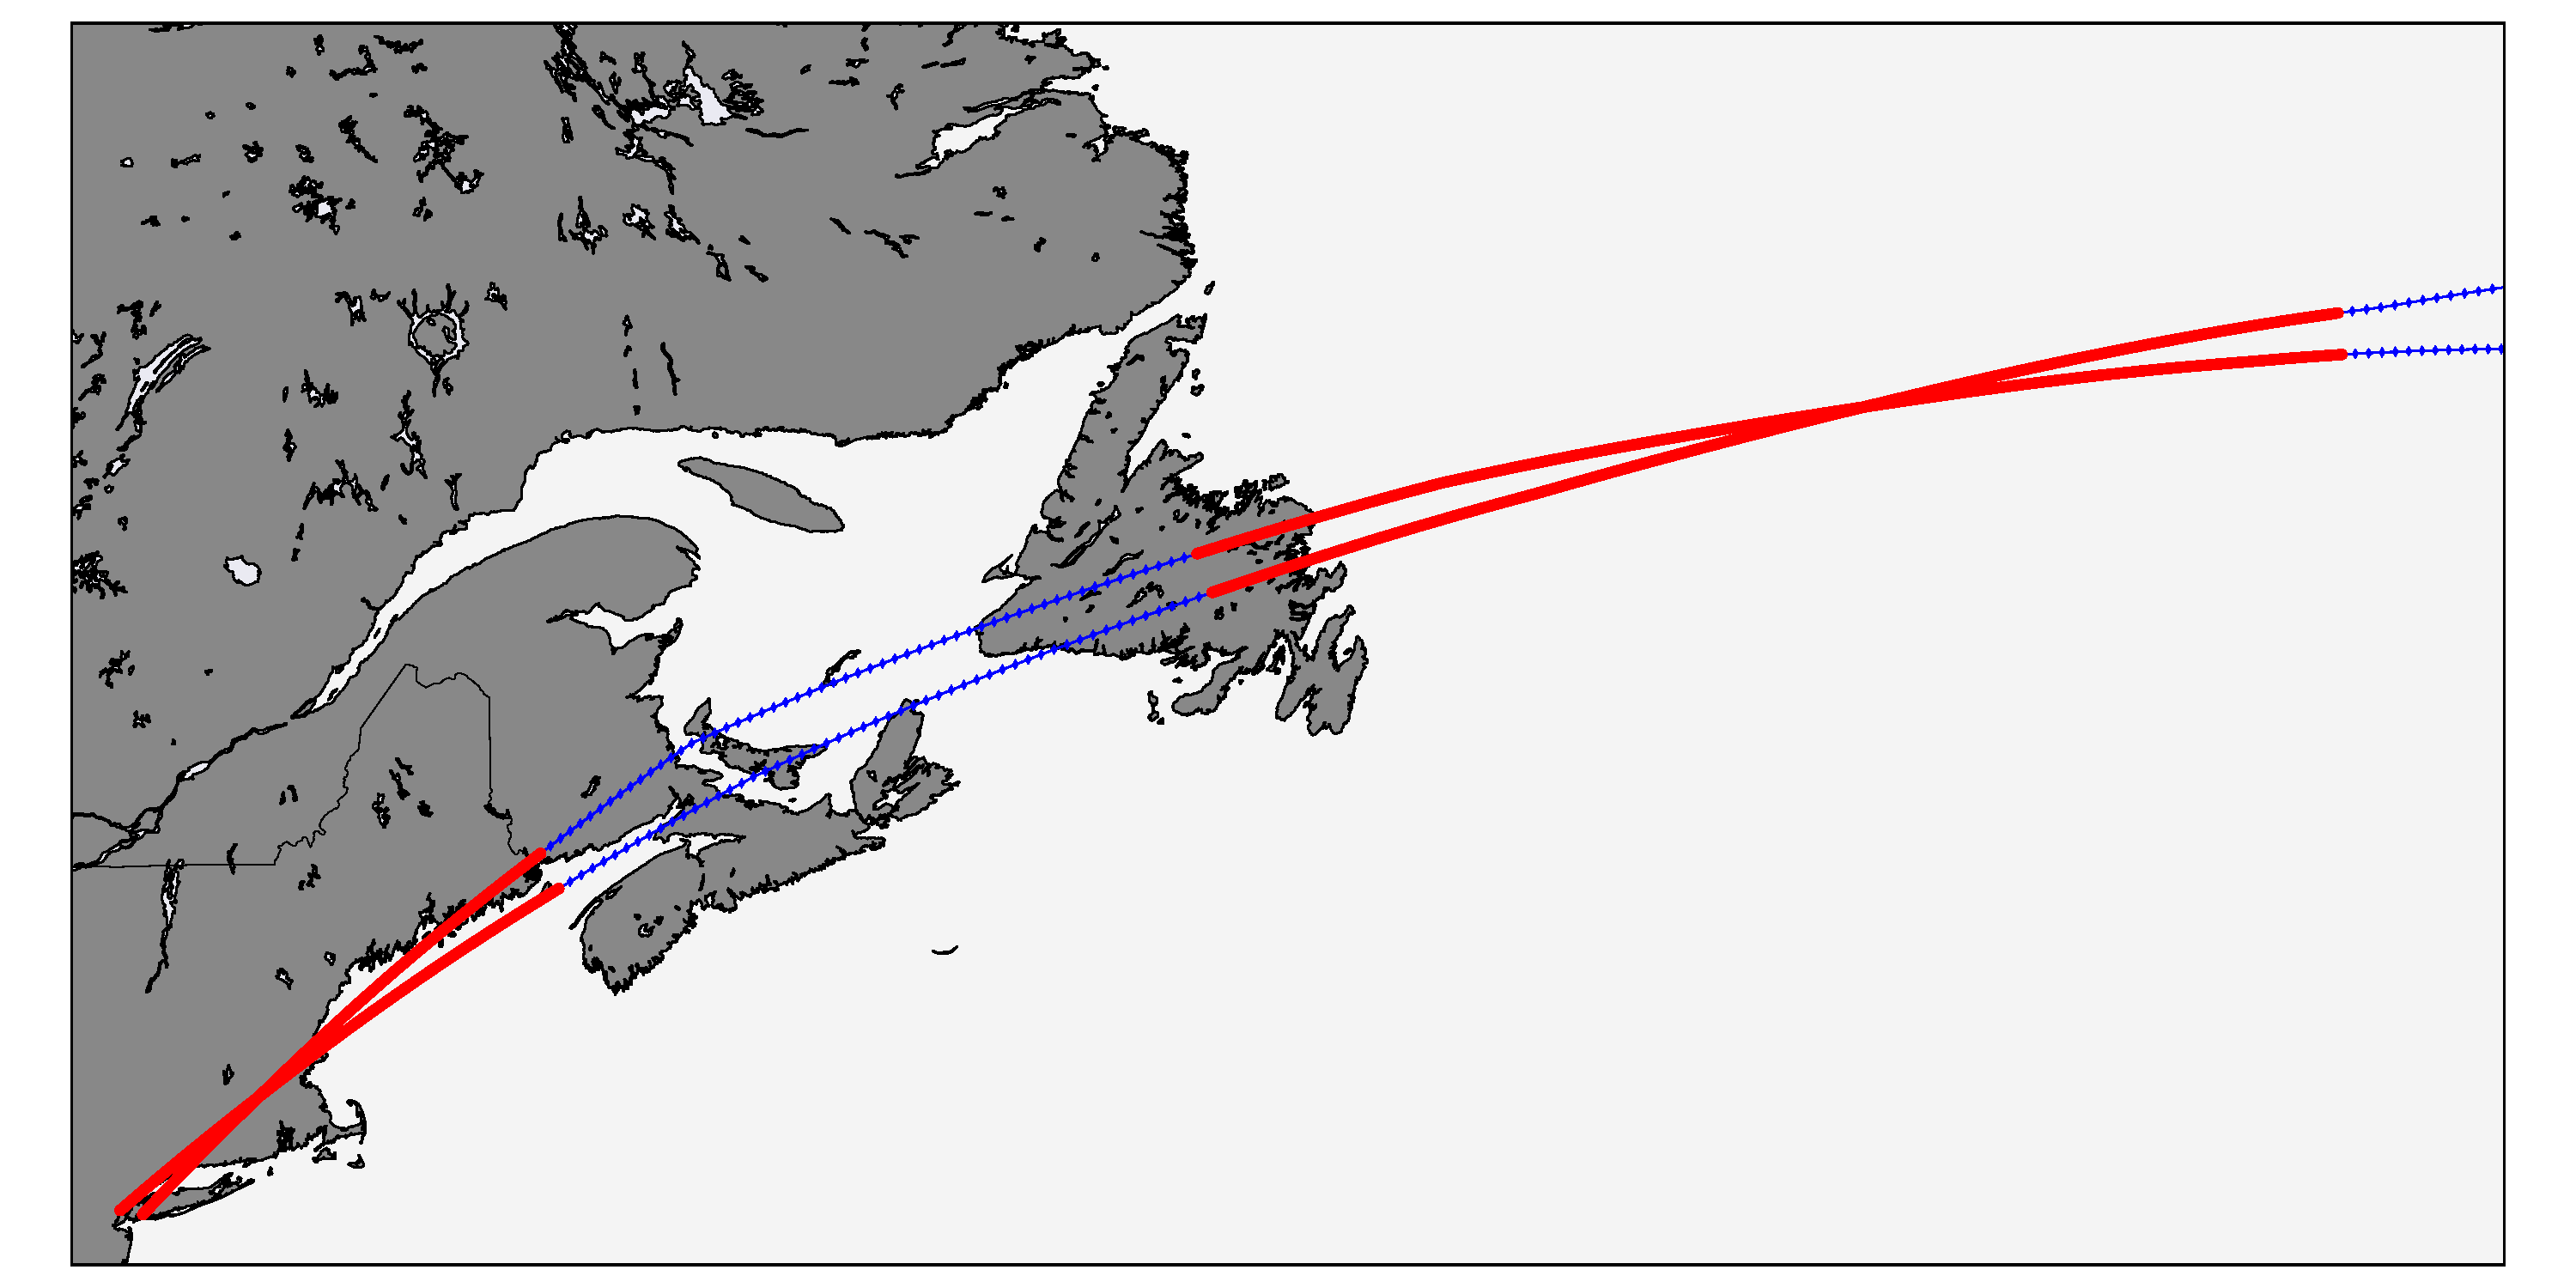
\includegraphics[width=0.45\textwidth,natwidth=1,natheight=0]{./pics/example_conflict_in_real_space.pdf}
    \end{center}
    \caption{Example of two parallel potential conflicts between two transatlantic flights starting from the east cost of the USA.}
    \label{fig:example_parallel_conflict}
\end{figure}

For a given pair of flights $(i, j)$ there might be multiple ``disjoint`` subsets in $C^{ij}_\parallel$
\begin{equation*}
    \bigcup_{n} C^{ij}_{\parallel n} = C^{ij}_\parallel
\end{equation*}
where
\begin{align*}
    & |t - s| \geq \Delta'_t \land |t' - s'| \geq \Delta'_t \\
    & \forall (x_{i, t},  x_{j, t'}) \in C^{ij}_{\parallel n}, \\
    & \forall (x_{i, s},  x_{j, s'}) \in C^{ij}_{\parallel n'}, \\
    & n \neq n' \; .
\end{align*}
In figure \ref{fig:example_parallel_conflict} an example of two separated clusters are shown.
Together with the remaining, spatially isolated, conflicting trajectory points
\begin{equation*}
    C^{ij}_{\times} = C^{ij}_0 \setminus C^{ij}_\parallel \; ,
\end{equation*}
these subsets of trajectory point clusters are called \emph{potential conflicts}.
\begin{equation*}
    C_k \in C = \{ C^{ij}_{\parallel n} | \forall i, j, n\} \cup  \{C^{ij}_{\times} | \forall i, j\}
\end{equation*}
Here, we introduced a conflict index $k\in\{1, \dots, N_c\}$, with $N_c = |C|$.
For each conflict index $k$, we will denote the pair of involved flights by $I_k = (i_k, j_k)$.

\begin{figure}[t]
    \begin{center}
        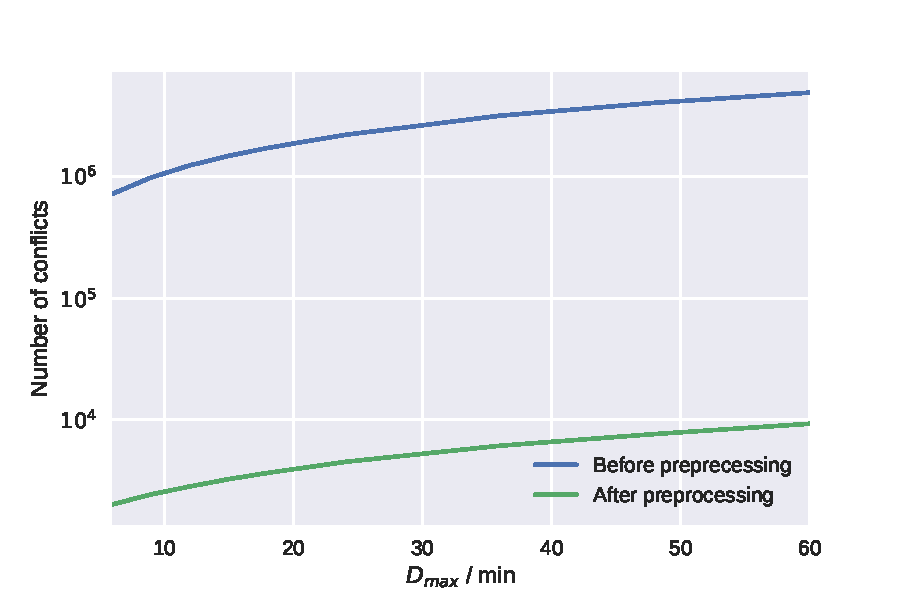
\includegraphics[width=0.45\textwidth,natwidth=1,natheight=0]{./pics/preprocessing_reduction_number_of_conflicts.pdf}
    \end{center}
    \caption{Preprocessing: Reduction in the number of potential conflicts for various upper delay bounds $D_\text{max}$.}
    \label{fig:preprocessing_reduction_number_of_conflicts}
\end{figure}

Before the preprocessing, the number of conflicts was given by $N_c^\text{before} = \sum_{ij} |C^{ij}_0|$.
As one can see in figure \ref{fig:preprocessing_reduction_number_of_conflicts} the preprocessing reduces the number of conflicts by orders of magnitude.

%%%%%%%%%%%%%%%%%%%%%%%%%%%%%%%%%%%%%%%%%%%%%%%%%%%%%%%%%%%%%%%%%%%%%%%%%%%%%%
%%%%%%%%%%%%%%%%%%%%%%%%%%%%%%%%%%%%%%%%%%%%%%%%%%%%%%%%%%%%%%%%%%%%%%%%%%%%%%
%%%%%%%%%%%%%%%%%%%%%%%%%%%%%%%%%%%%%%%%%%%%%%%%%%%%%%%%%%%%%%%%%%%%%%%%%%%%%%
\subsection{Conflict Avoidance}
In order to avoid conflicts, a flight $i$ can be either delayed at departure time by $d_i$ or by maneuver introduced delays $d_{ik}$ for each conflict $k$ the flight is involved in.
With this, the trajectory times of flight $i$ are shifted
\begin{align}
    t & \to t  + D_i(t) \; , \notag \\
    D_i(t) & = d_i + \sum_{k\in K_{i}(t)} d_{ik} \label{eqn:time_dependent_delay} \; , 
\end{align}
where $D_i(t)$ is the delay of flight $i$ at time $t$ and the sum runs over all the conflicts which are before $t$
\begin{equation*}
    K_{i}(t) = \left\{k \; |  \; \exists x_{i, t'} \in C_k \text{ for which } t' < t  \right\}  \; .
\end{equation*}
We introduce the pairs of times of spatially conflicting points inside a conflict $k$:
\begin{equation*}
    T_k =  \{(t, t') \; | \; (x_{i, t}, x_{j, t'}) \in C_k , (i, j) \in I_k \} \; .
\end{equation*}
A conflicts $k$ between two flights $i$ and $j$ occurs if the delays are chosen such that a temporal difference between spatially conflicting points is below $\Delta_t$:
\begin{align*}
    & |t + D_i(t) - t' - D_j(t')| < \Delta_t \\
    \Rightarrow  & - \Delta_t - (t - t') < D_i(t) - D_j(t') < \Delta_t - (t - t') \; , 
\end{align*}
for any $(t, t') \in T_k$.
Hence a conflict $k$ is avoided if
\begin{equation*}
    D_i(t) - D_j(t') \notin D_k \qquad \forall \, (t, t') \in T_k \; .
\end{equation*}
with
\begin{equation*}
    D_k = \left(-\Delta_t - \max_{(t, t') \in T_k} (t - t'), \Delta_t - \min_{(t, t') \in T_k} (t - t')\right) \; .
\end{equation*}

%%%%%%%%%%%%%%%%%%%%%%%%%%%%%%%%%%%%%%%%%%%%%%%%%%%%%%%%%%%%%%%%%%%%%%%%%%%%%%
%%%%%%%%%%%%%%%%%%%%%%%%%%%%%%%%%%%%%%%%%%%%%%%%%%%%%%%%%%%%%%%%%%%%%%%%%%%%%%
%%%%%%%%%%%%%%%%%%%%%%%%%%%%%%%%%%%%%%%%%%%%%%%%%%%%%%%%%%%%%%%%%%%%%%%%%%%%%%
%%%%%%%%%%%%%%%%%%%%%%%%%%%%%%%%%%%%%%%%%%%%%%%%%%%%%%%%%%%%%%%%%%%%%%%%%%%%%%
%%%%%%%%%%%%%%%%%%%%%%%%%%%%%%%%%%%%%%%%%%%%%%%%%%%%%%%%%%%%%%%%%%%%%%%%%%%%%%
\section{Departure Delay Model}
\label{sec:departure_delay_model}
In this section we describe a simplified version of the above problem.
We restrict ourselves to departure delays and neglect maneuvers.
Hence the optimization problem can be written as
\begin{align}
    & \min_{d_i} \sum_i d_i \notag \\
    & \text{s.t.}  \quad 
    d_i - d_j \notin D_k \qquad \forall \, (t, t') \in T_k \label{eqn:departure_delay_model}
\end{align}

The problem needs to be mapped to a quadratic binary optimization problem (QUBO) in order to be solvable by a D-Wave quantum annealer.
As a first step, we introduce a discretization and upper bound for the departure delay variables 
\begin{equation*}
    d_i \in \{0, \Delta_d, 2\Delta_d, \dots, d_\text{max} \}\, ,
\end{equation*}
where $d_\text{max} = N_d \Delta_d$ and $(N_d + 1)$ is the number of delay steps.
With this we can write the departure delay variables in terms of new binary variables $d_{i\alpha}$ by
\begin{align}
    d_i & = \sum_\alpha \alpha d_{i\alpha} \notag \\
    \alpha & \in \{0, \Delta_d, 2\Delta_d, \dots, d_\text{max} \}\, . \label{eqn:departure_delay_model_discretization}
\end{align}
However, this approach requires $\sum_\alpha d_{i\alpha} = 1$ to have a unique representation of $d_i$ by $d_{i\alpha}$.
This is achieved by adding the following contribution to the QUBO
\begin{equation*}
    Q_\text{unique} = \lambda_\text{unique} \sum_i \left( \sum_\alpha d_{i\alpha} - 1 \right)^2 \; .
\end{equation*}
where $\lambda_\text{unique}$ is a penalty weight sufficiently large to ensure $Q_\text{unique}=0$ for the solution.
The cost function in \eqref{eqn:departure_delay_model} yields contribution
\begin{equation*}
    Q_\text{delay} = \frac{1}{d_\text{max}}\sum_{i\alpha} \alpha d_{i\alpha} \; ,
\end{equation*}
where we have chosen the prefactor $1/d_\text{max}$ for convenience.
The last contribution to the QUBO represents the conflict avoidance
\begin{equation*}
    Q_\text{conflict} = \lambda_\text{conflict} \sum_k \sum_{(\alpha, \beta) \in A_k} d_{i\alpha} d_{j\alpha} \biggl. \biggr|_{i, j \in I_k}
\end{equation*}
where $A_k$ is the set of all $(\alpha, \beta)$ which correspond to a conflict
\begin{equation*}
    A_k = \{(\alpha, \beta) \; | \; \alpha - \beta \in D_k\}
\end{equation*}
Again, $\lambda_\text{conflict}$ is the penalty weight for this contribution which have to be chosen large enough to ensure $Q_\text{conflict}=0$ for the solution.
The total QUBO of the departure delay model then reads
\begin{equation*}
    Q_\text{DDM} = Q_\text{delay} + Q_\text{unique} + Q_\text{conflict}
\end{equation*}

%%%%%%%%%%%%%%%%%%%%%%%%%%%%%%%%%%%%%%%%%%%%%%%%%%%%%%%%%%%%%%%%%%%%%%%%%%%%%%
%%%%%%%%%%%%%%%%%%%%%%%%%%%%%%%%%%%%%%%%%%%%%%%%%%%%%%%%%%%%%%%%%%%%%%%%%%%%%%
%%%%%%%%%%%%%%%%%%%%%%%%%%%%%%%%%%%%%%%%%%%%%%%%%%%%%%%%%%%%%%%%%%%%%%%%%%%%%%
\subsection{Natural Subsets of the Problem}
To investigate the problem we consider each flight as a vertex of a graph and each conflict between two flights as an edge of this graph.
The connected components of this \emph{conflict graph} represent natural subsets of the problem.

%%%%%%%%%%%%%%%%%%%%%%%%%%%%%%%%%%%%%%%%%%%%%%%%%%%%%%%%%%%%%%%%%%%%%%%%%%%%%%
%%%%%%%%%%%%%%%%%%%%%%%%%%%%%%%%%%%%%%%%%%%%%%%%%%%%%%%%%%%%%%%%%%%%%%%%%%%%%%
%%%%%%%%%%%%%%%%%%%%%%%%%%%%%%%%%%%%%%%%%%%%%%%%%%%%%%%%%%%%%%%%%%%%%%%%%%%%%%
\subsection{Configuration Space Restrictions}
It is important to understand how the restrictions to the configuration space by \eqref{eqn:departure_delay_model_discretization} influence the solution quality.
Therefore we solve \eqref{eqn:departure_delay_model} with a constraint programming solver \cite{numberjack} for various delay discretizations and upper bounds as well as for the continuous problem.
As problem instances we used most of the connected components of the conflict graph for $D_\text{max}=18$ minutes with up to $N_f=50$ flights and $N_c=104$ conflicts.
\begin{figure}[htpb]
    \centering
    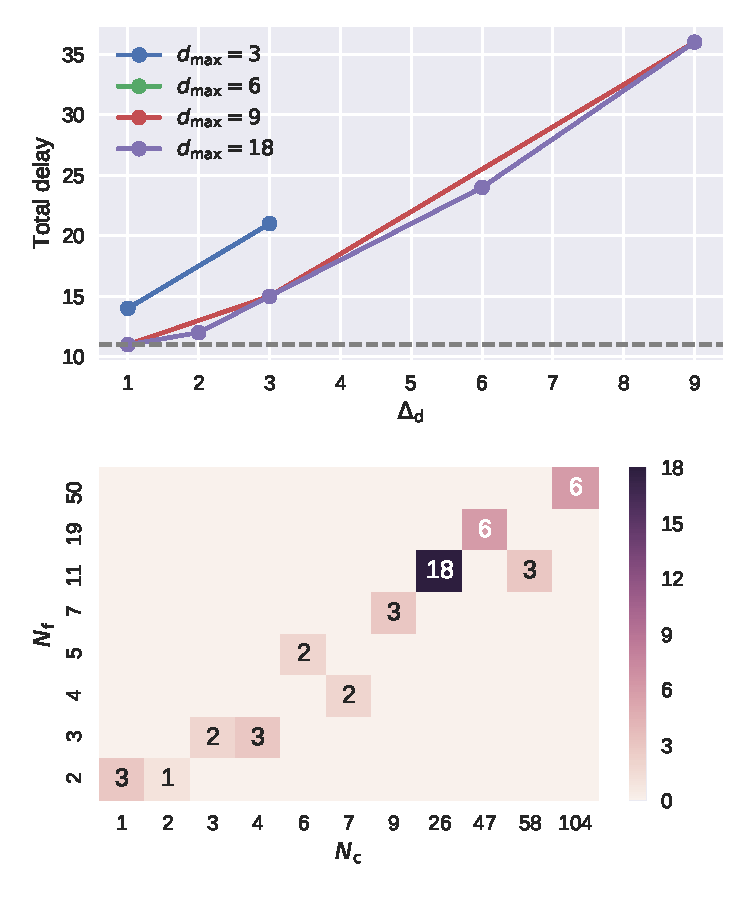
\includegraphics[width=0.45\textwidth,natwidth=1,natheight=0]{./pics/delay_only_cp_results.pdf}
    \caption{Top: Total delay of constraint programming solutions for a problem instance with $N_f=19$ flights and $N_c=47$ conflicts for various discretization parameters.
    Bottom: Minimum $d_\text{max}$ which yield optimal solution in continuous problem for various problem instances. For all problem instances we used $D_\text{max}=18$ minutes.}
    \label{fig:delay_only_cp_results}
\end{figure}

In figure \ref{fig:delay_only_cp_results} one can see the results for a problem instance extracted from a connected component of the conflict graph with $N_f=19$ flights and $N_c=47$ conflicts.
With the exception of the small maximum delay $d_\text{max} = 3$ min, the total delay of the solutions is nearly independent of the maximum delay.
Moreover it is monotonically increasing with the coarseness of the discretization.
Since the original data is discretized in time in units of $1$ minute, $\Delta_t=1$ yield the same result as a continuous variable with the same upper bound.
Obviously the total delay for the continuous solution decreases monotonically with $d_\text{max}$.
Above a certain value $d^0_\text{max}$ the total delay stays the same.
With one exception, we found that for all the investigated problem instances $d^0_\text{max}\leq6$ minutes (see figure \ref{fig:delay_only_cp_results}).
Therefore we conclude, that a moderate maximum delay is sufficient even for larger problem instances.
On the other hand, the delay discretization should be as fine as possible to obtain a high quality solutions.
%%%%%%%%%%%%%%%%%%%%%%%%%%%%%%%%%%%%%%%%%%%%%%%%%%%%%%%%%%%%%%%%%%%%%%%%%%%%%%
%%%%%%%%%%%%%%%%%%%%%%%%%%%%%%%%%%%%%%%%%%%%%%%%%%%%%%%%%%%%%%%%%%%%%%%%%%%%%%
%%%%%%%%%%%%%%%%%%%%%%%%%%%%%%%%%%%%%%%%%%%%%%%%%%%%%%%%%%%%%%%%%%%%%%%%%%%%%%
\subsection{Choice of the Penalty Weights}
\begin{figure}[htpb]
    \centering
    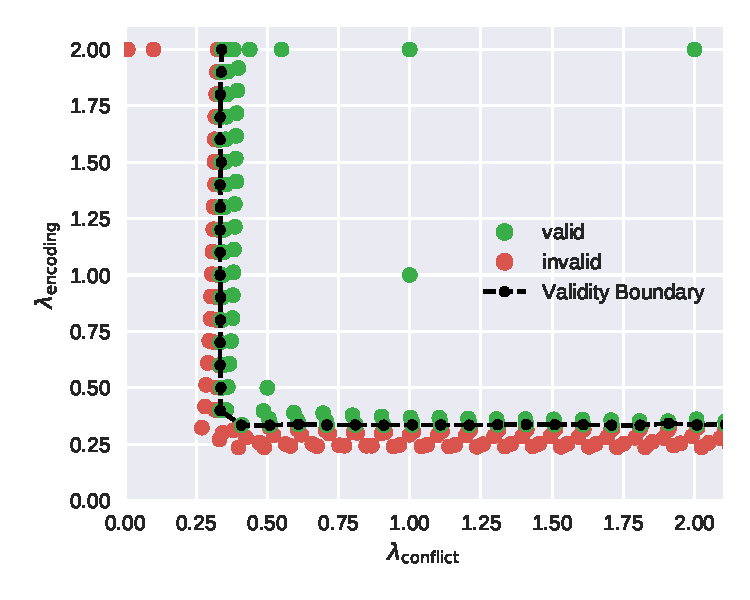
\includegraphics[width=0.45\textwidth,natwidth=1,natheight=0]{./pics/validity_boundary_example.pdf}
    \caption{Validity of exact solution to a QUBO extracted from a a problem instance with $N_f=7$ flights and $N_c=9$ conflicts in dependence on the choice of the penalty weights, $\lambda_\text{unique}$ and $\lambda_\text{conflict}$.}
    \label{fig:penalty_weights}
\end{figure}
%%%%%%%%%%%%%%%%%%%%%%%%%%%%%%%%%%%%%%%%%%%%%%%%%%%%%%%%%%%%%%%%%%%%%%%%%%%%%%
%%%%%%%%%%%%%%%%%%%%%%%%%%%%%%%%%%%%%%%%%%%%%%%%%%%%%%%%%%%%%%%%%%%%%%%%%%%%%%
%%%%%%%%%%%%%%%%%%%%%%%%%%%%%%%%%%%%%%%%%%%%%%%%%%%%%%%%%%%%%%%%%%%%%%%%%%%%%%
\subsection{Results from ICM}
%%%%%%%%%%%%%%%%%%%%%%%%%%%%%%%%%%%%%%%%%%%%%%%%%%%%%%%%%%%%%%%%%%%%%%%%%%%%%%
%%%%%%%%%%%%%%%%%%%%%%%%%%%%%%%%%%%%%%%%%%%%%%%%%%%%%%%%%%%%%%%%%%%%%%%%%%%%%%
%%%%%%%%%%%%%%%%%%%%%%%%%%%%%%%%%%%%%%%%%%%%%%%%%%%%%%%%%%%%%%%%%%%%%%%%%%%%%%
\subsection{Embedding to D-Wave}
\begin{figure}[htpb]
    \centering
    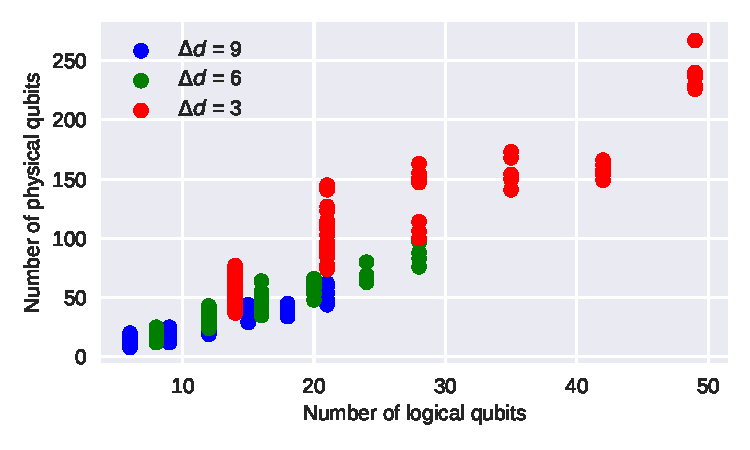
\includegraphics[width=0.45\textwidth,natwidth=1,natheight=0]{./pics/physicalVsLogicalNumberOfQubits.pdf}
    \caption{Number of physical qubits versus the number of logical qubits after embedding of QUBO instances with up to $N_f=50$ and $N_c=104$}
    \label{fig:number_of_physical_qubits}
\end{figure}
%%%%%%%%%%%%%%%%%%%%%%%%%%%%%%%%%%%%%%%%%%%%%%%%%%%%%%%%%%%%%%%%%%%%%%%%%%%%%%
%%%%%%%%%%%%%%%%%%%%%%%%%%%%%%%%%%%%%%%%%%%%%%%%%%%%%%%%%%%%%%%%%%%%%%%%%%%%%%
%%%%%%%%%%%%%%%%%%%%%%%%%%%%%%%%%%%%%%%%%%%%%%%%%%%%%%%%%%%%%%%%%%%%%%%%%%%%%%
\subsection{Quantum Annealing Results}
\begin{figure}[htpb]
    \centering
    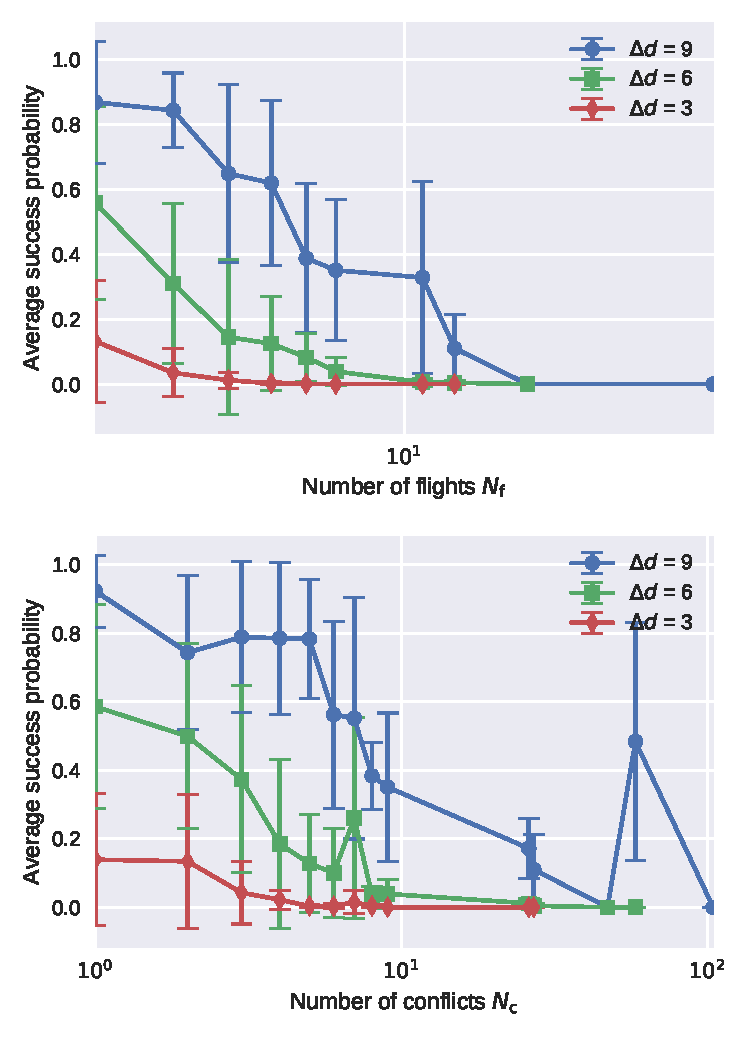
\includegraphics[width=0.45\textwidth,natwidth=1,natheight=0]{./pics/annealing_results_success_vs_flights_and_conflicts.pdf}
    \caption{Success probability for QUBO instances in dependence of the number of flights $N_f$ and the number of conflicts $N_c$. 
             The error bars indicate the standard deviation.
             We used $10000$ annealing runs for each instance and penalty weights $\lambda = \lambda_\text{conflict} = \lambda_\text{unique} \in \{0.5, 1, 2\}$. 
    }
    \label{fig:success_probability}
\end{figure}

%%%%%%%%%%%%%%%%%%%%%%%%%%%%%%%%%%%%%%%%%%%%%%%%%%%%%%%%%%%%%%%%%%%%%%%%%%%%%%
%%%%%%%%%%%%%%%%%%%%%%%%%%%%%%%%%%%%%%%%%%%%%%%%%%%%%%%%%%%%%%%%%%%%%%%%%%%%%%
%%%%%%%%%%%%%%%%%%%%%%%%%%%%%%%%%%%%%%%%%%%%%%%%%%%%%%%%%%%%%%%%%%%%%%%%%%%%%%
%%%%%%%%%%%%%%%%%%%%%%%%%%%%%%%%%%%%%%%%%%%%%%%%%%%%%%%%%%%%%%%%%%%%%%%%%%%%%%
%%%%%%%%%%%%%%%%%%%%%%%%%%%%%%%%%%%%%%%%%%%%%%%%%%%%%%%%%%%%%%%%%%%%%%%%%%%%%%
\section{Maneuver Model}
A more realistic model of the problem can be created by including maneuvers.
As mentioned above the maneuvers enter our formulation as additional delays $d_{ik}$ at the conflict time.
In the course of mapping to a QUBO formulation, we need to make sure to retain the combinatorial nature of the problem.
We do this by restricting the vast realm of maneuvers to two distinct choices:
Only one of the two involved flights is delayed while leaving the other flight untouched
\begin{equation} \label{eqn:maneuver_model_maneuver_decision}
    \text{if } d_{ik} \neq 0 \Rightarrow d_{jk} = 0  \qquad \forall (i, j) \in I_k \; \forall k \; .
\end{equation}
Moreover, we set the resulting maneuver delays to a constant value $d_M$ large enough to capture all kinds of real maneuvers.
A natural choice for this is the temporal conflict threshold $d_M = \Delta_t$.

With \eqref{eqn:time_dependent_delay} we can introduce the delay a flight $i$ at the conflict $k$ as
\begin{equation} \label{eqn:maneuver_model_delay_at_conflict}
    D_{ik} = d_i + \sum_{k'<k} d_{ik} \; ,
\end{equation}
where we have defined a temporal ordering of the conflicts for each flight $i$ by
\begin{align*}
                 &k < p \text{ if } t < t' \\
    \text{ for } &t = \operatorname*{arg\, min}_s x_{i, s} \in C_k \; , \\
                 &t' = \operatorname*{arg\, min}_s x_{i, s} \in C_p
\end{align*}

The departure delay variables are represented by binary variables as it was done in section \ref{sec:departure_delay_model}.
The maneuver delays are given by
\begin{equation*}
    d_{ik} = d_M a_{ik} \qquad a_{ik} \in \{0, 1\}
\end{equation*}
Since the total delay is given by $\sum_{ik} D_{ik}$, we can write the corresponding QUBO contribution as
\begin{equation*}
    \tilde Q_\text{delay} = \sum_{i\alpha} \alpha d_{i\alpha}  + \sum_{ik} d_M a_{ik}\; ,
\end{equation*}

For the conflict avoidance, we need to introduce another variable representing the delay at a given conflict
\begin{equation*}
    D_{ik} = \sum_\delta \delta \Delta_{ik\delta} \qquad \Delta_{ik\delta} \in \{0, 1\} \; .
\end{equation*}
By restricting ourselves to $\Delta_d = \Delta_t$ the values of $\delta$ in the above equation are given as
\begin{equation*}
    \delta \in \{0, \Delta_t, 2\Delta_t, \dots,  (N_d + M_{ik}) \Delta_t\} \; .
\end{equation*}
Here, $M_{ik}$ is the number of conflicts the flight $i$ is involved in before $k$.
In order to fulfill \eqref{eqn:maneuver_model_delay_at_conflict} we add the following contribution to the QUBO
\begin{equation*}
    \tilde Q_\Delta = \lambda_\Delta \sum_{ik}  \left( \sum_{\alpha} \alpha d_{i\alpha}  + \sum_{k'<k} d_M a_{ik'} - \sum_\delta \delta \Delta_{ik\delta}\right)^2 \biggl. \biggr|_{i, j \in I_k}
\end{equation*}
For unique representation of the variables we add 
\begin{align*}
    \tilde Q_\text{unique} = \lambda_\text{unique} & \left\{  \sum_i \left( \sum_\alpha d_{i\alpha} - 1 \right)^2 \right. \\
                      & \left. + \sum_{ik} \left( \sum_\delta \Delta_{ik\delta} - 1 \right)^2 \right\} \; .
\end{align*}
Conflicts are avoided if $D_{ik} - D_{jk} \notin D_k$, $(i, j) \in I_k$. 
The corresponding QUBO contribution reads
\begin{equation*}
    \tilde Q_\text{conflict} = \lambda_\text{conflict} \sum_k \sum_{(\delta, \delta') \in B_k} \Delta_{ik\delta} \Delta_{jk\delta'} \biggl. \biggr|_{i, j \in I_k}
\end{equation*}
where $B_k$ is the set of all $(\delta, \delta')$ which correspond to a conflict
\begin{equation*}
    B_k = \{(\delta, \delta') \; | \; \delta - \delta' \in D_k\}
\end{equation*}
The penalty weights $\lambda_\Delta$, $\lambda_\text{unique}$ and $\lambda_\text{conflict}$ must be chosen large enough to ensure vanishing contributions from the corresponding QUBO terms for the solution.

Finally, the maneuver decision described by \eqref{eqn:maneuver_model_maneuver_decision} is incorporated by a antiferromagnetic coupling between the two maneuver delay variables
\begin{equation*}
    \tilde Q_\text{maneuver} = J \sum_k  \left( s_{ik} s_{jk} + 1\right)_{i, j \in I_k} \; .
\end{equation*}
with 
\begin{equation*}
    s_{ik} = 2 a_{ik} - 1 \in \{-1, 1\}
\end{equation*}
and $J>0$ has to be chosen large enough. 
A solution is considered to be valid only if $\tilde Q_\text{maneuver} = 0$.
Hence, the total QUBO for the maneuver model reads
\begin{equation*}
    Q_\text{MM} = \tilde Q_\text{delay} + \tilde Q_\Delta  + \tilde Q_\text{unique} + \tilde Q_\text{conflict} + \tilde Q_\text{maneuver} 
\end{equation*}

\bibliography{atm}

\end{document}
